\documentclass[twoside,a4paper]{article}

\usepackage{graphicx}
\usepackage{url}
\usepackage{verbatim}
\usepackage{tikz}
\usetikzlibrary{arrows,shapes}

\title{ Multimodal recommender engine based on Apache Mahout and Apache Solr }
\author{
	Author \\
	Lukas Hofmaier \\
	lukas.hofmaier@hsr.ch
 	\and
	Supervisors \\
        Hansj''org Huser
}
\date{
	\textsc{University of Applied Sciences Rapperswil}\\
	Project Thesis,
	\today
}
\begin{document}
\maketitle
\tableofcontents

\section{Introduction}
\label{sec:intro}

\subsection{Recommender engines}
\label{sec:recommenderengines}

Recommender engines are services that recommend articles (items) to users based on their past actions. They attempt to infer taste and preferences. A recommender engine presents the user previously unknown items that are of interest for the user. 

For example, if a user has purchased the movies "Terminator 2" and "Transformers" the recommender engine will present the activ user a list of other similar movies.

E-commerce sites that deploy a recommender engine can have a increase in sales of 8 - 13 percent \footnote{http://www.practicalecommerce.com/articles/1942-10-Questions-on-Product-Recommendations}.

\subsection{Strategies}
\label{sec:strategies}

There are different strategies to discover to recommend a user new items \cite{Owen}.
\begin{description}
\item[Collaborative Filtering] This strategy is only based on the preference or taste information from many users. For example, a recommender engine based on collaborativ filtering uses the ratings of all users to compute the similarity between all items. 

It requires no knowledge of the properties of the items. Recommender engines based on collaborative filtering do not care what the items are and what attributes they have. This can be an advantage because the same technique can be applied to different types of items. 

User preferences will change over time. Another advandage is that collaborative filtering will update the model automaticaly as it's exposed to new user histories. The systems learns.
\item[Content based filterting] Content-based recommendation techniques use attributes of the items in order to predict preferences of users. For example, if a recommender recommends movies of a Steven Spielberg because the active user likes other movies of Steven Spielberg it uses content based filtering.
\end{description}

This article describes a recommender engine based on collaborative filtering. The recommendations are only based on user input. The recommender engine is designed to mixe any number of user actions (clicks, purchases, likes, tags). The ratings of a user and the applied tags will be used to compute recommendations.

\subsection{Challenges and Problems}

There are serveral ways to design and build a recommender eninge \cite{Dunning14}.

\begin{itemize}
\item Design a custom recommender engine. That approach requires a team of highly trained engineer and data scientist.
\item Use products that offer drag-and-drop approaches. Some of these product try to automaticaly select the right algorithms. This recommender engines aren't very effective and a most of the effort required is put into getting the data into the right format.
\item Use the service of a high-end machine-learning consultancy. These companies achieve effective results by trying a huge collection of algorithms at each problem and selecting the algoritm that gives the best result.
\end{itemize}

There are several problem and challenges in building a recommender engine:
\begin{itemize}
\item Many algorithms relies on user ratings. Ratings come from a subset of users. Only user who like to rate will rate items. 
\end{itemize}

In this article we use a simplified approach to the recommender problem described in \cite{Dunning14}. The goal of the apporach presented in this article is to provide a simple solutions that gives the user practical recommendation. There are academic approaches that produce recommendation with a smaller error but these require complex mathematical models. The goal of the apporach presented in this article is to provide a simplified, general solution for the recommender problem. In contrast to an academic approach it is easiear to extend the recommender engine to a multimodel recommender.


Many existing collaborativ filtering type recommenders use one user activity to model preference \cite{ferrel}. But a variety of user activities can be use in combination to improve the quality of recommendations. Section \ref{sec:design} will describe how different type of interactions is used as input data to train the recommender.

The recommender described in this article is divided in two parts.
\begin{itemize}
\item Computation of simililarity and the update of the text search engine is done offline, ahead of time.
\item Recommendations are generated instantly by quering the text search eninge using rescents actions of the user.


\end{itemize}

\subsection{Overview}

Section \ref{sec:design} will describe the design of the co-occurence based recommender. The similiarity metric log-likelihood ratio is described and a short introduction for the search engine Apache Solr is given.


\section{Co-occurence based multimodal recommender}
\label{sec:cooccurence}

The recommender design we discuss will use the histories of users behavior to compute the similarity between all items. We use co-occurence to compute the similarity of two items. The recommenders looks up items that appear in the recent user history and presents the user a list with similar items.

All movies are stored as documents in a database (we use Apache Solr). The documents contain metainformation (e.g. title, tags, genre) about the items in fields. The fields are indexed by a search engine and made searchable.

In addidion the document has indicator fields. Indicator fields contain id's of that are found to be worth recommending in the co-occurence analysis.

\tikzset{
 mynode/.style={rectangle,rounded corners,draw=black, top color=white, bottom color=yellow!50,very thick, inner sep=1em, minimum size=3em, text centered}
}
\tikzstyle{format} = [draw, thin, fill=blue!20]
\tikzstyle{medium} = [ellipse, draw, thin, fill=green!20, minimum height=2.5em]
\begin{figure}
\centering
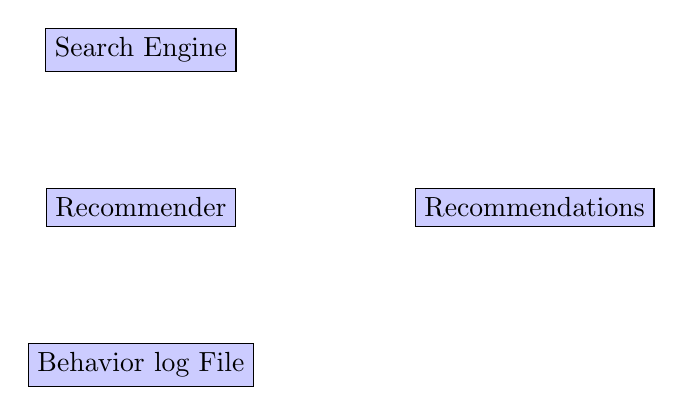
\begin{tikzpicture}[node distance=20mm,
data/.style={
rectangle,
draw,
thin,
fill=blue!20
}]
\node (recommender) [data] {Recommender};
\node (topn) [data,right of = recommender, node distance=50mm] {Recommendations};
\node (history) [data,below of = recommender] {Behavior log File};
\node (db) [data,above of= recommender] {Search Engine};
\end{tikzpicture}
\caption{Recommender engine}
\end{figure}

The described design has the following benefits
\begin{itemize}
\item Exploit existing search engine technology.
\item The search engine can be used for conventional search as well.
\item Users can use search engine to search for metadata.
\item Recommender engine can be extended with additional indicators.
\end{itemize}

\subsection{Log-likelihood similarity}
\label{sec:llr}

In order to compute the similarity between two items we use co-occurence or the log likelihood similarity.
Co-occurence in the context of recommender systems describes the circumstance that two items are similar when the same users interact (like, purchase, etc) interact with them.

The co-occurence based recommender uses the user history in order to make recommendations. The user history doesnt contains explicit preference values. Explicit user preferences are ratings of a user for an item. The user history only contains interactions of users and items. 

We can use various user actions to compute the similarity of two items. For example:
\begin{itemize}
\item Purchase action
\item Click action
\item The user might click on a like button for evrey item
\end{itemize}

 The log-likelihood similiarity is based on the number of users (or tags) in common between two items. According to \cite{Dunning93} the log-likelihood similiarity is suitable for data that only captures the interaction and no preference between users and items. 

Compared to the Jaccard coefficient \cite{Hartung} the log-likelihood-based similarity computes higher similarites for anomalous co-occurences than for items that occur in every user history. The log-likelihood similarity  is the probability that two users share the same items due to chance. For a detailed explanation of the math involved see \cite{Dunning93}. 

We describe the log-likelihood-based similarity with a small example dataset. Suppose we analyse the following web log of user purchases represented as a table (see appendix of raw web log).

\begin{table}
\begin{center}
\begin{tabular}{rllll}
 & 101 & 102 & 103 & 104\\
1 & x & x & x & \\
2 & x &  & x & x\\
3 & x & x & x & \\
4 &  & x & x & x\\
5 & x & x & x & x\\
\end{tabular}
\end{center}
\caption{Example dataset. The columns represent the user interaction with an item. Items are named 1 - 4 and users 101 - 104}
\label{tbl:llr}
\end{table}

Table \ref{tbl:llr} shows the purchases of four users for five items. The items are represented with ids 1-4 and the users with ids 101 - 104.
In the example dataset of table \ref{tbl:llr} the items 1 and 2 are similar because they purchased the same items. 

In order to get the similarity between all items we compute the log-likelihood ratio strength for every item pair. This will produce a $5 \times 5$ indicator matrix. Table \ref{tab:indicatormatrix} shows the indicator matrix for the sample dataset from table \ref{tbl:llr}

\begin{table}
  \centering
\begin{center}
\begin{tabular}{rrrrrr}
 & 1 & 2 & 3 & 4 & 5\\
1 &  & 0.40 & 0.81 & 0.63 & 0\\
2 & 0.40 &  & 0.40 & 0.63 & 0\\
3 & 0.81 & 0.40 &  & 0.63 & 0\\
4 & 0.63 & 0.63 & 0.63 &  & 0\\
5 & 0 & 0 & 0 & 0 & \\
 &  &  &  &  & \\
\end{tabular}
\end{center}
  \caption{Indicator matrix for item purchases}
  \label{tab:indicatormatrix}
\end{table}


Allthoug item 5 share all users with item 1 and 3, the log-likelihood ratio is 0. Every user purchased item 5. It would not be interesting to recommend item 5 to a user because it is to obious.
\subsection{Apache Solr}
\label{sec:solr}

Solr is a search engine that is optimized to search large volumes of text-centric data and return results sorted by relevance. It is built on Apache Lucene, an information retrieval library.

A reason why we deploy a search engine is that the application is read-dominant. The recommender will query the data far more often than it will create new documents or update the indicators. Solr is optimized to for executing queries as opposed to storing data.

Solr stores the documents in a flat structure.

Solr return documents sorted in descending order by a score that indicates the strength of the match of the document to the query. In a relational database a row either mathces a query or it does not.

The reason why we deploy a search engine in order to make recommendations is that Solr scores documents based on the presence of query terms in the document similar to a recommendations engine based on the presence of indicator.

Solr is able to parse text streams. It extract the structure and make it searchable.

\subsection{Apache Spark}
\label{sec:spark}
\verb|spark-rowsimilarity| is a script that comes with spark. It takes as input a text file representation of a matrix of sparse vectors. It finds similar rows. The input is in text-delimited form where there are three delimiters used. By default it reads (rowID<tab>columnID1:strength1<space>columnID2:strength2...) The job only supports LLR similarity. This job only supports LLR similarity.
The input has the following format:
\begin{verbatim}
1	1
2	2
3	3 
\end{verbatim}


\section{Evaluation}
\label{sec:evaluation}
Recommenders answer the question "What are the best recommendations for a user?". If we want to evaluate a recommender, we have to define, what's a "good" recommendation.
Some recommender predict the preferences of a user. One possibility to evaluate a recommender is to calculate the difference between the estimated preference and the actual preference.

Those actual prefences don't exist. Nobody knows how a user likes some new item in the future.
But we can simulate the prefencences of the future by setting aside a small part of the real data set as test data. These preferences aren't present in the training data set. Instead the recommender predicts the preferences for the missing test data set and the estimates are compared to the actual values.

Another approach to evaluate a recommender is to take a broader view of the recommender problem. It's not strictly necessary to estimate preference values in order to produce recommendations. In many cases presenting a ordered list of recommendations is sufficient. The list is ordered from best to worst recommendation.


\subsection{Dataset}
\label{sec:dataset}

This dataset used in this project describes rating and free-text tagging activity from MovieLens, a movie recommendation service \cite{movielensdata}.
MovieLens data sets were collected by the GroupLens Research Project at the University of Minnesota.
 
This data set consists of:
\begin{itemize}
\item 100,000 ratings (1-5) from 943 users on 1682 movies. 
\item Each user has rated at least 20 movies. 
\end{itemize}

The data was collected through the MovieLens web site (movielens.umn.edu) during the seven-month period from September 19th, 
1997 through April 22nd, 1998.

All selected users had rated at least 20 movies.
All ratings are contained in the file ratings.csv. Each line of this file after the header row represents one rating of one movie by one user, and has the following format:

\begin{verbatim}
userId,movieId,rating,timestamp.
\end{verbatim}

All tags are contained in the file $tags.csv$. Each line of this file after the header row represents one tag applied to one movie by one user, and has the following format:
\begin{verbatim}
userId,movieId,tag,timestamp
\end{verbatim}

\subsection{Movielens}
\label{sec:movielens}

The MovieLens dataset describes 5-star rating and free-text tagging activity from MovieLens, a movie recommendation service. It contains 100023 ratings and 2488 tag applications across 8570 movies. These data were created by 706 users 


\subsection{Precision and Recall}
\label{sec:precision}


\begin{description}
\item[Precision] Precision is the proportion of top results that relevant. Suppose the recommender recommends 5 items. If 3 items are good recommendations then the precision is $3/5$.
\item[Recall] Recall is the proportion of good recommendations that appear in the recommendation result. Suppose there are 9 good recommendations. If the recommender results contains 3 of these good recommendations then the recall is 3/9.
\end{description}

In order to calculate precision and recall the implementation determines the top \verb|n| preferences for each user. It removes those preferences from the data model. It evaluates precision and recall with the new data model. It calculates a top-N recommendation list for each user and compares it with the real top-N preferences.

The evaluation process has the following paramters:
\begin{description}
\item[Size of the result] The number of recommendations to consider. The length of the recommendation list.
\item[Relevance] Determines if an item is relevant or not.
\end{description}


\subsection{Baseline Algorithm}
\label{sec:baselinealgorithm}


\section{Multimodalrecommender}
\label{sec:multimodalrecommender}

The recommender has the follwowing parameters:
\begin{itemize}
\item The number of ratings or tags that are used for the query.
\end{itemize}

\subsection{Results}
\label{sec:results}


\subsection{Example data set}
\label{sec:exampledataset}

The example data set is a small set of user preferences. It has constructect properties:
\begin{itemize}
\item Items 108, 109 und 111 are similiar.
\item User 9 likes the items 111, 109 

\end{itemize}

\section{Conclusion}
\label{sec:similarity}

A large amount of work was required to convert formats between the user logs the Apache Mahout and Apache Solr.

\section{Infrastructur}
\label{sec:infrastructur}

\appendix

\section{Sample Input Data}
\label{sec:sampleinput}

\begin{verbatim}
itemid, userid, timestamp
1,101,980730861
1,102,980731380
1,103,980731926
2,101,980732037
2,103,980730408
2,104,980731766
3,101,980731282
3,102,980730769
3,103,980731208
4,102,980732235
4,103,980731417
5,101,980731745
5,102,980731621
5,103,980731417
5,104,980731208
\end{verbatim}

\section{Case Study: artoffer.ch}
\label{sec:artoffer}

The following action are used as indicators
\begin{itemize}
\item When a user visits the page of a item. (boolean)
\item When a user likes an item.
\item Tags
\end{itemize}
\bibliographystyle{plain}
\bibliography{a}
\end{document}
